\documentclass[border=0mm]{standalone}

\usepackage{contour}
\usepackage{ifthen}
\usepackage{tcolorbox}
\usepackage{tikz}
\usepackage{xcolor}

%%%%%%%%%%%%%%%%%%%%%%%%%%%%%%%%%%%%%%%%%%%%%%%%%%%%%%%%%%%%%%%%%%%%%%%%%%%%%
% File: colours.tex
% Author: Edmund Mulligan <edmund@edmundmulligan.name>
% Version: 1.0
% This file is part of the workbook for Non-Violent Communication.
% Description: Contains the definitions of the colours used in the workbook.
%%%%%%%%%%%%%%%%%%%%%%%%%%%%%%%%%%%%%%%%%%%%%%%%%%%%%%%%%%%%%%%%%%%%%%%%%%%%%
\definecolor{tem_cyan}{rgb}{.2, .8, .8}
\definecolor{tem_purple}{rgb}{0.706, 0.051, 0.831}
\definecolor{tem_grey}{RGB}{245, 245, 245}

 \definecolor{tem_blue1}{RGB}{240,248,255} % AliceBlue
 \definecolor{tem_blue2}{RGB}{135,206,250} % LightSkyBlue
 \definecolor{tem_blue3}{RGB}{100,149,237} % CornflowerBlue
 \definecolor{tem_blue4}{RGB}{0,0,255}     % Blue
 \definecolor{tem_blue5}{RGB}{0,0,128}     % Navy


\begin{document}
  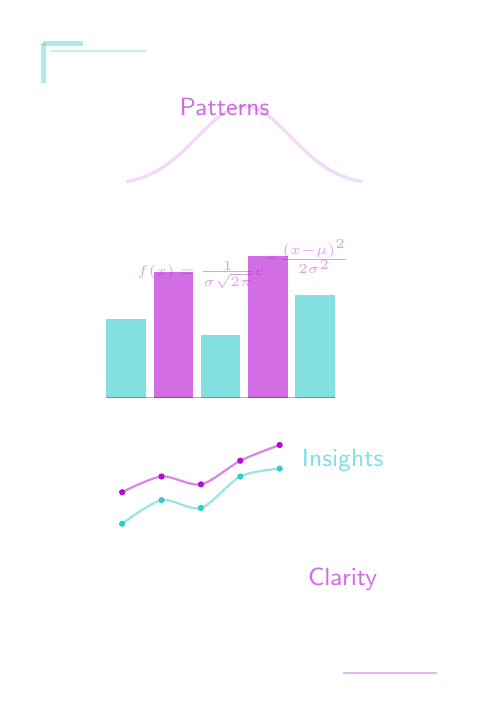
\begin{tikzpicture}
    % Portrait dimensions: 55mm x 85mm (approx 5.5cm x 8.5cm)
    % Define the card background
    \fill[white] (0,0) rectangle (5.5,8.5);
    
    % Bell curve (normal distribution) in background - iconic and recognizable
    \begin{scope}[transparency group, opacity=0.15]
      \draw[tem_purple, very thick, smooth, samples=100, domain=-2.5:2.5] 
        plot ({2.75 + 0.6*\x}, {6.5 + 1.0*exp(-\x*\x/2)});
    \end{scope}
    
    % Simple bar chart visualization (clean and accessible)
    \begin{scope}[shift={(1.0,3.8)}]
      \fill[tem_cyan, opacity=0.6] (0,0) rectangle (0.5,1.0);
      \fill[tem_purple, opacity=0.6] (0.6,0) rectangle (1.1,1.6);
      \fill[tem_cyan, opacity=0.6] (1.2,0) rectangle (1.7,0.8);
      \fill[tem_purple, opacity=0.6] (1.8,0) rectangle (2.3,1.8);
      \fill[tem_cyan, opacity=0.6] (2.4,0) rectangle (2.9,1.3);
      % Base line
      \draw[black, opacity=0.3] (0,0) -- (2.9,0);
    \end{scope}
    
    % Clean line graph
    \begin{scope}[shift={(1.2,2.2)}]
      \draw[tem_cyan, thick, opacity=0.5] 
        plot[smooth] coordinates {(0,0) (0.5,0.3) (1.0,0.2) (1.5,0.6) (2.0,0.7)};
      \draw[tem_purple, thick, opacity=0.5] 
        plot[smooth] coordinates {(0,0.4) (0.5,0.6) (1.0,0.5) (1.5,0.8) (2.0,1.0)};
      % Data points
      \foreach \x/\y in {0/0, 0.5/0.3, 1.0/0.2, 1.5/0.6, 2.0/0.7} {
        \fill[tem_cyan] (\x,\y) circle (0.04);
      }
      \foreach \x/\y in {0/0.4, 0.5/0.6, 1.0/0.5, 1.5/0.8, 2.0/1.0} {
        \fill[tem_purple] (\x,\y) circle (0.04);
      }
    \end{scope}
    
    % Normal distribution PDF formula (closer to bell curve)
    \node[tem_purple, font=\tiny, opacity=0.4, align=center] at (2.75, 5.5) 
      {$f(x) = \frac{1}{\sigma\sqrt{2\pi}} e^{-\frac{(x-\mu)^2}{2\sigma^2}}$};
    
    % Simple friendly labels (no complex notation)
    \node[tem_purple, font=\small\sffamily, opacity=0.6] at (2.5, 7.5) {Patterns};
    \node[tem_cyan, font=\small\sffamily, opacity=0.6] at (4.0, 3.0) {Insights};
    \node[tem_purple, font=\small\sffamily, opacity=0.6] at (4.0, 1.5) {Clarity};
    
    % Subtle decorative elements suggesting data flow
    \draw[tem_cyan, thick, opacity=0.3] (0.3,8.2) -- (1.5,8.2);
    \draw[tem_purple, thick, opacity=0.3] (4.0,0.3) -- (5.2,0.3);
    
    % Small corner accent
    \draw[tem_cyan, line width=2pt, opacity=0.4] (0.2,8.3) -- (0.2,7.8);
    \draw[tem_cyan, line width=2pt, opacity=0.4] (0.2,8.3) -- (0.7,8.3);
    
  \end{tikzpicture}
\end{document}
